\documentclass[12pt]{article}

\usepackage[utf8]{inputenc}
\usepackage[T1]{fontenc}
\usepackage{microtype}
\usepackage{amsmath,amssymb}
\usepackage{geometry}
\usepackage{hyperref}
\usepackage{setspace}
\usepackage{tikz}
\usetikzlibrary{shapes,positioning,calc}

\geometry{margin=1in}
\onehalfspacing
\emergencystretch=1em

\title{The Mathematics of Oppression:\\A Set-Theoretic Framework for Analyzing Systems of Domination}
\author{}
\date{}

\begin{document}

\maketitle

\begin{abstract}
This paper develops a formal mathematical framework for analyzing systems of oppression using set theory, discrete mathematics, and historical analysis. The framework identifies four architectural components common to all oppressive systems: (1) asymmetric autonomy restriction between In-groups and Out-groups, (2) selective empathy that validates In-group suffering while dismissing Out-group harm, (3) ideological justification through spurious claims, and (4) resistance to structural critique. Through detailed analysis of American racism---from slave patrols to mass incarceration---I demonstrate that the Out-group targeted by systemic oppression \textit{expands} over time, progressively encompassing groups once part of the In-group. This expansion reveals that oppressive systems serve not the nominal In-group but an Elite class ($E \subset I$) that uses division to prevent solidarity. To demonstrate the framework's generality, I briefly examine how identical mathematical structures manifest at the micro-relational level in asymmetric intimate relationships. The transferability of this architecture across scales---from macro-level racial systems to micro-level relational dynamics---suggests that oppression operates through recognizable, formalizable patterns that can be identified and resisted across contexts.
\end{abstract}

\section{Introduction}

This paper proposes a mathematical framework for understanding systems of oppression---social arrangements that systematically disadvantage one group (the Out-group, $O$) while advantaging another (the In-group, $I$). Traditional analyses of oppression often focus on individual prejudice or specific policy outcomes. However, such approaches fail to capture the \textit{structural} dimensions of oppression: the recurring patterns, the self-reinforcing mechanisms, and the remarkable consistency of design across different systems and scales.

The central thesis of this paper is that systems of oppression share a common \textbf{architecture of control}---a formal structure that can be identified mathematically regardless of the specific groups involved or the historical context. This architecture consists of:
\begin{enumerate}
    \item \textbf{Asymmetric autonomy restriction}: Policies and norms that constrain the Out-group's freedom while preserving the In-group's
    \item \textbf{Selective empathy}: Validation of In-group suffering while dismissing or pathologizing Out-group harm
    \item \textbf{Ideological justification}: Narratives that naturalize the asymmetry through spurious claims
    \item \textbf{Resistance to structural critique}: Mechanisms that deflect analysis from the system to individual behavior
\end{enumerate}

To develop and validate this framework, I examine \textbf{racism} as the primary case study---specifically, the American system of racial oppression from its colonial origins to the present. Racism provides an ideal test case because of its extensive historical documentation, its clear policy mechanisms, and its ongoing relevance. Through set-theoretic analysis, I demonstrate that racism exhibits all four architectural components and, crucially, that the Out-group has \textit{expanded} over time rather than contracted.

This expansion reveals a deeper truth: the system does not ultimately serve the racial In-group but rather an Elite class ($E \subset I$) that uses racial division to prevent cross-group solidarity. The ``wages of whiteness''---psychological compensation for poor whites---substitute for material advancement while the Elite extract value from both groups.

To demonstrate that this framework applies beyond macro-level racial systems, I briefly examine how identical mathematical structures manifest in \textbf{asymmetric intimate relation\-ships}---a phenomenon analyzed in detail in companion work on Pseudo-Hybrid Asymmetric Monogamy (PHAM). The transferability of oppressive architecture across scales---from geopolitical systems to intimate relationships---suggests that oppression operates through recognizable patterns that can be formalized and resisted.

\textbf{A critical methodological note}: Comparing the \textit{architecture} of different oppressive systems does not equate their \textit{phenomenology}. This paper analyzes design principles---how asymmetry is created, justified, and maintained---not magnitudes of suffering. Recognizing shared structure illuminates how systems of domination reproduce themselves; it does not diminish the unique gravity of any particular manifestation.

\subsection{Racism as Primary Example}

\textbf{The Problem with Traditional Definitions}

Traditional definitions of racism reveal a troubling pattern: they relegate the systemic dimension to secondary or tertiary status, often buried as the third or fourth definition in dictionaries---the ``cliff notes'' version that few people encounter or use. Consider typical definitional hierarchies:

\begin{enumerate}
    \item \textbf{Primary definition}: Individual prejudice or discrimination based on race
    \item \textbf{Secondary definition}: Belief in racial superiority
    \item \textbf{Tertiary definition} (if present at all): Systemic or institutional discrimination
\end{enumerate}

This ordering is not merely unfortunate---it is \textbf{fundamentally backwards}. By centering individual prejudice, these definitions obscure the cardinal reality: \textit{the systemic element is the primary operation}. The interpersonal manifestations---individual prejudice, discriminatory actions, racial animus---are \textit{downstream products} created to maintain the systemic structure, not the cause of it.

\textbf{Reversing the Causal Arrow}

The conventional framing suggests this causal relationship:
\[
\text{Individual Prejudice} \rightarrow \text{Discriminatory Actions} \rightarrow \text{Systemic Outcomes}
\]

This implies that if we eliminate individual prejudice, systemic racism will disappear. But history reveals the opposite causal structure:
\[
\text{Elite Economic Interests} \rightarrow \text{Systemic Racialization} \rightarrow \text{Interpersonal Prejudice}
\]

As demonstrated in Section 2, interpersonal racism---the attitudes, beliefs, and prejudices held by individuals---\textit{was deliberately created to justify and maintain the systemic structure}. Zurara's racialization of Africans as subhuman was not a spontaneous expression of Portuguese prejudice; it was commissioned work designed to justify a system of unlimited exploitation. The interpersonal followed the systemic, not vice versa.

\textbf{The Linguistic Evidence}

Moreover, traditional definitions overlook a fundamental linguistic aspect: the suffix ``-ism'' in ``racism'' already denotes a \textit{system}. We recognize this in other contexts:
\begin{itemize}
    \item \textbf{Capitalism}: A \textit{system} of economic organization, not just individual acts of trade
    \item \textbf{Feudalism}: A \textit{system} of social hierarchy, not just individual lord-serf relationships
    \item \textbf{Colonialism}: A \textit{system} of territorial exploitation, not just individual acts of conquest
\end{itemize}

Yet with racism, we persistently treat it as a collection of individual attitudes rather than recognizing the systemic nature embedded in the very structure of the word. This is not accidental---it serves to deflect attention from the structural mechanisms that create and perpetuate racial inequality.

\textbf{The Critical Distinction: Racism is Not Prejudice}

This analysis reveals a fundamental conceptual error in conflating racism with prejudice or bias. The distinction is not one of degree but of \textit{kind}:

\begin{quote}
\textbf{Prejudice or bias}: Individual attitudes, stereotypes, or discriminatory behaviors based on group membership. These are interpersonal phenomena that can exist in any direction and between any groups.

\textbf{Racism}: A \textit{system of oppression} that weaponizes prejudice and bias into structural mechanisms of exploitation and control. Racism takes individual prejudice and transforms it through institutionalization into a self-perpetuating apparatus that serves Elite economic interests.
\end{quote}

\textbf{Without the systemic element, there is no racism---there is only prejudice.} The system is not an optional feature or a more severe manifestation; it is the \textit{defining characteristic} that distinguishes racism from generic bias. Consider:

\begin{itemize}
    \item A person holding negative stereotypes about another group = \textbf{prejudice}
    \item A system that codifies those stereotypes into law, policy, and institutional practice to extract labor and prevent solidarity = \textbf{racism}
\end{itemize}

Racism is the process of taking interpersonal prejudice and bias---which exist across all human societies---and \textbf{weaponizing them} into a system that:
\begin{enumerate}
    \item \textbf{Institutionalizes} prejudice through policy ($P$)
    \item \textbf{Concentrates} harm at the intersection $O_{\text{racialized}} \cap P$
    \item \textbf{Naturalizes} the resulting disparities through ideology
    \item \textbf{Compounds} disadvantage over time through the mechanisms described in Section 3
    \item \textbf{Serves} Elite economic interests by preventing working-class solidarity
\end{enumerate}

This distinction has profound implications. An individual can hold prejudices without participating in racism if those prejudices are not institutionalized into systems of power. Conversely, an individual can participate in and benefit from racist systems even while holding no conscious prejudice---because racism operates \textit{systemically}, through policies and structures, not merely through individual attitudes.

The conflation of racism with prejudice is not merely imprecise---it is \textbf{functionally useful to the system}. By treating them as synonymous, we:
\begin{itemize}
    \item Suggest that eliminating individual prejudice eliminates racism
    \item Enable individuals to disavow racism by disavowing prejudice
    \item Obscure the structural mechanisms that create and maintain racial hierarchy
    \item Deflect attention from the Elite class that benefits from racial division
    \item Make structural analysis seem like an overreaction to individual attitudes
\end{itemize}

The system is \textit{the point}. Racism is fundamentally and irreducibly systemic. Without the system, we're discussing prejudice, bias, or discrimination---real phenomena, but categorically different from racism as a system of oppression.

\textbf{Why the Misdirection Matters}

Centering individual prejudice as the primary definition of racism accomplishes several functions that protect the systemic structure:

\begin{enumerate}
    \item \textbf{Individualizes responsibility}: If racism is primarily individual prejudice, then solutions focus on changing hearts and minds rather than dismantling structures.
    
    \item \textbf{Obscures Elite benefits}: Individual-focused definitions hide the fact that racism serves Elite economic interests by preventing working-class solidarity.
    
    \item \textbf{Enables plausible deniability}: Individuals can claim ``I'm not racist'' (meaning ``I don't hold personal prejudice'') while participating in and benefiting from racist systems.
    
    \item \textbf{Makes structural critique seem extreme}: If racism is ``just'' individual prejudice, then analyzing systemic structures appears to be overreach or ``seeing racism everywhere.''
    
    \item \textbf{Perpetuates the system}: By misidentifying the disease (treating symptoms rather than cause), individual-focused definitions ensure the system persists.
\end{enumerate}

\textbf{The Correct Hierarchy}

A proper definition must reverse the conventional ordering:

\begin{enumerate}
    \item \textbf{Primary}: Racism is a \textit{system} of policies and structures that create and maintain racial hierarchies for Elite economic benefit
    \item \textbf{Secondary}: This system is justified through ideological narratives that naturalize racial categories and hierarchies
    \item \textbf{Tertiary}: These narratives manifest in interpersonal prejudices and discriminatory actions that reinforce the system
\end{enumerate}

This ordering reflects the historical reality established in Section 2: systemic racialization came first, ideological justification followed, and interpersonal prejudice was cultivated to maintain the structure. The interpersonal is real and harmful, but it is \textit{epiphenomenal}---a surface manifestation of the deeper systemic operation.

To address this fundamental gap in conventional definitions, I propose a new definition that places the systemic element where it belongs: at the center of analysis. This definition emphasizes racism as a system of oppression, deeply rooted in historical practices and policies that categorize individuals based on perceived racial differences---a system deliberately created by Elites to break class solidarity and maintain exploitable labor.

\section{Historical Context}

\subsection{Portuguese Class Dynamics and the Elite's Dilemma}

Before understanding the invention of race, we must first understand the class dynamics that necessitated it. In 15th century Portugal, as in much of medieval Europe, society had achieved a degree of class solidarity that constrained Elite exploitation. The feudal system, while hierarchical, operated within a shared moral framework: all humans, regardless of status, were part of the same moral community. Peasants and nobility alike were Christians, subjects of the same crown, and---critically---recognized as human beings with souls.

This moral inclusion created practical limits on exploitation. While the Elite could extract labor through serfdom and taxation, they faced constraints:
\begin{itemize}
    \item \textbf{Religious doctrine}: The Catholic Church, despite supporting hierarchy, imposed limits on the treatment of Christians. Enslavement of fellow Christians was prohibited or heavily restricted.
    \item \textbf{Legal protections}: Even serfs had some legal standing---they could not be killed arbitrarily, families could not be separated at will, and certain customary rights were recognized.
    \item \textbf{Social cohesion}: Shared identity as Portuguese, as Christians, and as humans created bonds that could translate into solidarity against Elite overreach.
    \item \textbf{Demographic limits}: The available labor pool consisted of people who belonged to the moral community, limiting how brutally they could be exploited without risking rebellion or moral condemnation.
\end{itemize}

The Portuguese Elite faced a fundamental problem: \textbf{how to create a permanent slave class without violating the moral framework that constrained exploitation of the existing population}. They needed a labor force that could be worked to death, families that could be separated, and people who could be treated as property---all without triggering the moral and legal protections that applied to humans.

The solution was elegant and horrifying: \textbf{remove an entire category of people from the moral community by declaring them non-human}.

\subsection{The Invention of Race as Moral Exclusion}

The concept of race and the systemic nature of racism have their roots deeply embedded in this Elite need to break class solidarity and create a slave class unconstrained by moral limits. A pivotal figure in this narrative is Gomes de Zurara, whose work in the 1450s laid the groundwork for the racialization of African peoples. Commissioned by the Portuguese monarchy, Zurara authored a chronicle that justified the enslavement of African individuals by portraying them as a monolithic group, inherently inferior and \textit{subhuman}. 

This was not merely prejudice---it was \textbf{ontological exclusion}. Zurara's narrative did not simply claim Africans were inferior humans; it positioned them as \textit{a separate species}, more akin to animals than people. This act of lumping together the diverse peoples of Africa into a single, derogatory category represented an unprecedented move towards institutionalizing race as a basis for systemic oppression.

Dr.\ Ibram X.\ Kendi highlights Zurara's role in inventing race and racism, noting that his descriptions were instrumental in justifying the Portuguese slave trade. Zurara's narrative served not only as a moral and intellectual justification for the kidnapping and enslavement of African people but also set a precedent for European engagement with sub-Saharan Africa. Portugal, thus, became the first European nation to sail directly to sub-Saharan Africa for the purpose of capturing human beings for enslavement.

\subsection{The Implicit Contract: Securing Working-Class Complicity}

The racialization of Africans as subhuman created an \textbf{implicit contract} between the Elite and the Portuguese working class---a contract that would be replicated across Europe and the Americas:

\begin{quote}
\textit{``You may be poor, you may be exploited, but you will never be slaves. Your children will never be slaves. We do not enslave humans, and these Africans are not human---they are a subspecies, no different from cattle. Therefore, there is no reason not to exploit their labor, and your humanity is secured by their exclusion from humanity.''}
\end{quote}

This contract accomplished several objectives for the Elite and established what we term \textbf{slave capitalism}---a distinct economic model that combined capitalist accumulation with racialized slave labor:

\begin{enumerate}
    \item \textbf{Broke class solidarity}: Portuguese workers could no longer identify with enslaved Africans as fellow laborers because Africans were defined as non-human. Any solidarity based on shared exploitation was severed by the ontological divide.
    
    \item \textbf{Created psychological compensation}: Poor Portuguese gained status not through material improvement but through racial categorization. The ``wages of whiteness'' (though the term would emerge later) began here: your poverty matters less when you are assured you belong to the human race and others do not.
    
    \item \textbf{Eliminated moral constraints}: By removing Africans from the moral community, the Elite eliminated the religious, legal, and social protections that constrained exploitation. Africans could be worked to death, families could be torn apart, children could be sold---none of the protections afforded to humans applied.
    
    \item \textbf{Secured labor expansion}: The Elite gained access to a theoretically unlimited labor supply that could be brutally exploited without triggering the moral frameworks that protected Portuguese workers.
    
    \item \textbf{Prevented future solidarity}: The racial framework ensured that even if African-descended peoples gained freedom, the ontological divide would persist, preventing alliances between exploited groups across racial lines.
\end{enumerate}

\textbf{Defining Slave Capitalism}

The critical insight is that \textbf{slave capitalism did not end with industrial capitalism}---rather, industrial capitalism \textit{is} slave capitalism, merely evolved and geographically dispersed. The distinction between "historical slave capitalism" and "modern industrial capitalism" is a convenient fiction that obscures continuity. Modern capitalism remains fundamentally dependent on unfree labor and racialized exploitation, characterized by:

\begin{itemize}
    \item \textbf{Racialized property relations}: Human beings categorized as non-human become property, creating a form of capital accumulation based on ownership of people---continues through prison labor (13th Amendment exception) and debt bondage
    
    \item \textbf{Unlimited extraction}: Removal from moral community permits extraction without constraint---labor, reproduction, life itself become commodifiable. This continues through:
    \begin{itemize}
        \item \textbf{U.S. prison labor}: The 13th Amendment's "except as punishment for crime" clause enables legal slavery of 2.3 million incarcerated people working for \$0.14-\$0.63/hour
        \item \textbf{African resource extraction}: Western corporations exploit African labor at below-subsistence wages to extract raw materials (cobalt, coltan, lithium, rare earth minerals) essential for modern technology
        \item \textbf{Neocolonial contracts}: Former colonial powers (especially France) use debt, military pressure, and institutional capture to force African nations into exploitative resource contracts
    \end{itemize}
    
    \item \textbf{Generational perpetuation}: Children inherit enslaved status---modern manifestation: children of incarcerated parents are 6x more likely to be incarcerated; generational poverty traps families in exploited labor positions
    
    \item \textbf{Economic interdependence}: The entire Western economic system depends on slave labor, now geographically dispersed:
    \begin{itemize}
        \item Smartphones require cobalt mined by enslaved/child labor in Congo
        \item Electronics require rare earth minerals extracted through exploitative labor
        \item Fast fashion depends on sweatshop labor in Global South
        \item Agricultural supply chains rely on trafficked and bonded labor
    \end{itemize}
    
    \item \textbf{Elite accumulation}: Wealth concentrates in Elite class (now multi\-national corporations and billionaires) while working-class complicity is purchased through racial/national status rather than material improvement
\end{itemize}

\textbf{The Geographic Displacement Strategy}

What changed after formal abolition was not the elimination of slavery but its \textbf{geographic displacement} and legal obfuscation:

\begin{enumerate}
    \item \textbf{Domestic prison slavery}: 13th Amendment explicitly permits enslavement as criminal punishment, creating prison-industrial complex
    \item \textbf{Export slavery to Africa}: After centuries of extracting African bodies as slaves, capitalism now extracts African labor \textit{in situ}---keeping the exploitation in Africa while extracting the value
    \item \textbf{Neocolonial economic entrapment}: Former colonial powers use structural adjustment, debt, and military coercion to maintain exploitative relationships
\end{enumerate}

\textbf{Case Study: France's Dependence on African Exploitation}

The contemporary crisis in French-African relations exposes this dependency. France's economy has long relied on:

\begin{itemize}
    \item \textbf{CFA Franc system}: 14 African nations forced to use currency controlled by French Treasury, requiring them to deposit 50-85\% of reserves in France, giving France de facto control over their monetary policy
    \item \textbf{Resource extraction contracts}: Uranium from Niger powers French nuclear plants (70\% of French electricity); France pays far below market rates under contracts established during colonial period
    \item \textbf{Military enforcement}: France maintains military bases across former colonies to protect these arrangements, intervening militarily whenever governments attempt to renegotiate
\end{itemize}

\textbf{The Current Collapse:} As of 2023-2024, multiple African nations (Niger, Mali, Burkina Faso, Gabon) have expelled French military, rejected CFA Franc, and nationalized resources. France's economy is experiencing serious strain because:

\begin{itemize}
    \item Energy crisis: Without cheap Nigerien uranium, French nuclear power becomes economically unsustainable
    \item Loss of captive markets: CFA nations no longer forced to purchase French goods
    \item Capital flight: Without guaranteed extraction rights, French corporations lose massive revenue streams
    \item Inflation: France must now pay market rates for resources previously extracted at colonial prices
\end{itemize}

This demonstrates that \textbf{Western industrial capitalism would collapse without access to enslaved/exploited African labor and resources}. The system is not post-slavery; it is slavery with better PR.

\textbf{The Continuity of Slave Capitalism}

Therefore, slave capitalism is not "distinct from later industrial capitalism"---industrial capitalism \textit{is} slave capitalism that:
\begin{enumerate}
    \item Formally abolished chattel slavery in the West (while maintaining it via 13th Amendment loophole)
    \item Exported slavery back to Africa and Global South
    \item Used debt, structural adjustment, and military force to entrap African governments into exploiting their own people
    \item Extracts resources at significant deficits to source nations
    \item Maintains racial hierarchy globally (white Global North vs. racialized Global South)
\end{enumerate}

The model proved extraordinarily profitable for the Elite class, generating wealth accumulation at scales previously impossible under feudalism or wage labor systems---and it continues to do so through geographically dispersed but functionally identical slavery.

\subsection{The Global Replication of Slave Capitalism}

The Portuguese initiative was not an isolated endeavor but a starting point that led other European countries to follow suit. The adoption of Zurara's fictional portrayal of African inferiority by other European nations facilitated a widespread and systemic approach to viewing African peoples as commodities suitable for free labor. This marked the beginning of a systemic, global structure of \textbf{slave capitalism} that justified and perpetuated the exploitation and oppression of African peoples and their descendants.

The slave capitalism model proved so effective for Elite interests that it was replicated wherever European colonialism reached. Each iteration refined the system:
\begin{itemize}
    \item Spanish and British colonies adopted and expanded racialization
    \item Legal codes formalized racial categories (one-drop rule, blood quantum, etc.)
    \item Scientific racism emerged to provide pseudo-intellectual justification
    \item Religious institutions adapted theology to support racial hierarchy
    \item Financial systems developed around slave-based wealth (insurance, banking, mortgages on enslaved people)
\end{itemize}

\textbf{The Export to America: Slave Capitalism Crosses the Atlantic}

The model of slave capitalism was systematically exported to the American colonies, where it would become the economic foundation of the developing nation. This was not incidental but \textit{foundational}:

\begin{itemize}
    \item \textbf{Economic basis}: By 1860, enslaved people represented the largest single asset class in the United States, worth more than all manufacturing and railroads combined
    \item \textbf{Financial infrastructure}: Northern banks, insurance companies, and merchants profited enormously from financing and insuring the slave trade and slave-based production
    \item \textbf{Political power}: The Three-Fifths Compromise gave slave states disproportionate political representation by counting enslaved people for apportionment while denying them personhood
    \item \textbf{Legal codification}: State and federal law embedded slave capitalism into the legal structure, protecting it as property rights
\end{itemize}

The American implementation of slave capitalism would prove even more profitable and entrenched than its European origins, creating wealth that would finance the Industrial Revolution and establish the United States as an economic power.

\subsection{Institutional Legitimation: The Role of Church and Science}

The dehumanization of the African diaspora required more than political decree---it demanded \textbf{institutional legitimation} from society's most authoritative institutions. Both the Church and Science were enlisted, willingly or through institutional capture, to provide the moral and intellectual frameworks that naturalized the ontological exclusion of African peoples.

\textbf{The Church: Theological Justification for Ontological Exclusion}

The Catholic Church, despite its doctrine that all humans possess souls and are created in God's image, was systematically co-opted to support racialization:

\begin{enumerate}
    \item \textbf{The Curse of Ham doctrine}: Theologians reinterpreted the biblical story of Ham (Genesis 9:20-27) to claim that Africans were descendants of Ham, cursed by Noah to be ``servants of servants.'' This provided scriptural justification for enslavement specifically of African peoples.
    
    \item \textbf{Papal Bulls}: The Catholic Church issued explicit permissions for enslavement. The Dum Diversas (1452) authorized King Alfonso V of Portugal to ``invade, search out, capture, vanquish, and subdue all Saracens and pagans whatsoever'' and to ``reduce their persons to perpetual slavery.'' The Romanus Pontifex (1455) extended these rights, explicitly sanctioning the slave trade.
    
    \item \textbf{Baptism without liberation}: The Church maintained that baptizing enslaved Africans did not require their manumission. This theological innovation allowed simultaneous claims that Africans had souls (making conversion meaningful) while denying them the protections afforded to Christians---a contradiction resolved only by placing them in a separate onto\-logical category.
    
    \item \textbf{Missionary justification}: The enslavement of Africans was framed as a spiritual mercy---bringing ``pagans'' to Christianity justified their temporal bondage. This rationalization positioned exploitation as charitable work.
\end{enumerate}

The Church's role was critical because it provided \textit{moral authorization}. Without theological backing, the enslavement of fellow Christians would have triggered the very religious constraints the Elite sought to evade. By repositioning Africans as a separate category---cursed, pagan, subhuman---the Church enabled exploitation to proceed without violating Christian moral frameworks that protected the moral community.

\textbf{Science: Pseudo-Intellectual Justification through ``Racial Science''}

As Enlightenment values elevated empirical knowledge, Science became the new authority requiring capture. The development of ``scientific racism'' in the 18th-19th centuries provided secular justification for what theology had established:

\begin{enumerate}
    \item \textbf{Taxonomies of humanity}: Scientists like Carl Linnaeus (1735) and Johann Friedrich Blumenbach (1776) created racial classification systems that positioned Europeans as the superior ``race'' and Africans as closer to apes. These taxonomies were presented as empirical observations, not social constructions.
    
    \item \textbf{Craniology and phrenology}: Researchers like Samuel Morton measured skulls to ``prove'' African intellectual inferiority. These studies, though methodologically fraudulent, provided quantitative ``evidence'' that racialization reflected natural biological differences.
    
    \item \textbf{Polygenism}: Some scientists argued that different races were actually different \textit{species} with separate origins, directly contradicting Christian mono\-genesis but providing stronger justification for the claim that Africans were not fully human.
    
    \item \textbf{Social Darwinism}: Darwin's evolutionary theory was distorted to suggest that racial hierarchies reflected natural selection, with Europeans as more ``evolved.'' This naturalized exploitation as the inevitable outcome of biological superiority.
    
    \item \textbf{Eugenics}: By the late 19th-early 20th centuries, racial science had evolved into eugenics movements that advocated for ``racial purity'' and the prevention of ``degeneration'' through controlling reproduction of ``inferior races.''
\end{enumerate}

Scientific racism provided \textit{intellectual authorization}. It transformed what had been theological claims into ostensibly objective, empirical facts. When Science declared racial hierarchies to be natural biological realities, it became rational---even compassionate---to structure society according to these supposed natural laws.

\textbf{The Institutional Feedback Loop}

Church and Science did not merely justify the existing system---they created a \textbf{self-reinforcing feedback loop}:

\[
\begin{aligned}
&\text{Exploitation} \rightarrow \text{Observed disparities} \rightarrow \text{Theological/Scientific ``explanation''} \\
&\rightarrow \text{Naturalization} \rightarrow \text{Expanded exploitation}
\end{aligned}
\]

The brutal conditions of enslavement produced obvious disparities in wealth, health, and education. Rather than recognizing these as \textit{products} of the system, theologians and scientists framed them as \textit{evidence} of inherent African inferiority. This ``evidence'' then justified continued and expanded exploitation, which produced further disparities, which generated more ``evidence,'' and so on.

Both institutions also \textbf{trained the next generation}. Seminaries taught future clergy the theological justifications; universities taught future scientists, doctors, and policymakers the racial taxonomies. The dehumanization became embedded in education itself, ensuring its reproduction across generations.

\textbf{The Functional Necessity of Institutional Capture}

The Elite's capture of Church and Science was not incidental but \textit{functionally necessary} for three reasons:

\begin{enumerate}
    \item \textbf{Moral legitimacy}: The implicit contract with the working class required that African exclusion be \textit{morally justified}, not merely politically imposed. The Church provided this moral cover.
    
    \item \textbf{Intellectual legitimacy}: As education spread and Enlightenment values emphasized reason, exploitation required \textit{rational justification}. Science provided this intellectual cover.
    
    \item \textbf{Internalization}: For the system to be self-perpetuating, the dehumanization had to be \textit{internalized} as natural fact, not recognized as Elite strategy. When both God and Nature supposedly confirmed racial hierarchy, resistance seemed to oppose reality itself.
\end{enumerate}

The collaboration of Church and Science transformed racialization from a cynical political strategy into an apparently unchallengeable truth, backed by society's highest authorities on moral and empirical reality.

\subsection{Racism as Trojan Horse: Undermining the Constitution's Anti-Classist Framework}

The American Framers created a constitutional framework with explicitly anti-classist elements: prohibition of titles of nobility (Article I, Sections 9-10), grounding rights in ``the people'' rather than aristocratic privilege, and establishing equal protection principles. However, \textbf{the Framers had to compromise the democracy they were creating to uphold slavery}, introducing deliberate \textbf{contradictions}---``bugs in the source code''---that would allow the Elite to maintain class hierarchy while appearing to establish egalitarian governance.

These bugs were not accidental flaws but \textit{features} designed to preserve slave capitalism, and they have allowed American democracy to \textit{decay over time} as each generation exploits the same loopholes to expand the subjugated class.

\textbf{The Five Constitutional Bugs}

\begin{enumerate}
    \item \textbf{``We the People'' (undefined)}: Deliberately leaves this term undefined---creating a variable that can be narrowed to exclude disfavored groups. A deliberate vulnerability, not ambiguity.
    
    \item \textbf{No titles of nobility (with exception)}: Prohibits hereditary aristocracy but permits hereditary enslavement by framing it as property law rather than title law.
    
    \item \textbf{Equal representation (with inequality)}: One person, one vote---but counts enslaved people as 3/5 for apportionment while denying them personhood, embedding inequality into the equality mechanism.
    
    \item \textbf{Due process (with property exception)}: Protects against deprivation of ``life, liberty, or property''---but defines enslaved people as property, making the protection become the mechanism of oppression.
    
    \item \textbf{Commerce clause (enabling slave trade)}: Prohibits banning slave importation until 1808, explicitly protecting slave capitalism and establishing precedent that economic interests override human rights.
\end{enumerate}

These engineered vulnerabilities allow slave capitalism to persist within a framework claiming to oppose aristocracy.

\textbf{Dred Scott: Exploiting Bug \#1}

In \textit{Dred Scott v. Sandford} (1857), Chief Justice Taney demonstrated how Bug \#1 (undefined ``the people'') could be exploited. He excluded Black people from ``the people,'' declaring they ``had no rights which the white man was bound to respect,'' explicitly noting that inclusion would grant them the right to bear arms---``an outcome he found unacceptable.''

This revealed the four-step mechanism:
\begin{enumerate}
    \item Define racial classifications as natural facts (not social constructions)
    \item Exclude racialized groups from ``the people''
    \item Strip constitutional rights (rights depend on being among ``the people'')
    \item Evade anti-classist protections (frame as ``racial,'' not class-based)
\end{enumerate}

As the constitutional analysis brief notes: ``The phrase 'the people' is the constitutional hinge. If courts can narrow that definition... then every right dependent on that phrase becomes conditional. Conditional rights are not rights at all; they are privileges dispensed by the state.''

\textbf{The Pattern of Expansion and Democratic Decay}

Once these bugs existed, each generation exploited them to expand control:

\begin{itemize}
    \item \textbf{Bug \#1 (undefined ``the people'')}: Used by \textit{Dred Scott} to exclude Black people $\rightarrow$ now excludes felons, immigrants, political opponents
    \item \textbf{Bug \#4 (due process exception)}: Used to justify slavery $\rightarrow$ now justifies civil asset forfeiture, economic inequality
    \item \textbf{Bug \#5 (commerce primacy)}: Protected slave trade $\rightarrow$ now prioritizes corporate interests over human rights
\end{itemize}

The result: mass incarceration creates a ``criminal'' class excluded from ``the people''; economic policies concentrate wealth while dividing the working class along racial lines; surveillance state expansion by designating groups as ``dangerous''; gun control using \textit{Dred Scott}'s logic to narrow ``the people.''

\textbf{Why This Works: Racism as Elite Class Maintenance}

The genius of using racism to undermine anti-classist protections:
\begin{enumerate}
    \item \textbf{Appears natural}: Racial categories framed as biological facts, not social constructions serving Elite interests
    \item \textbf{Evades scrutiny}: Constitutional prohibitions on class hierarchy don't apply to ``natural'' racial differences
    \item \textbf{Divides resistance}: Working-class whites invested in racial hierarchy, preventing cross-racial solidarity
    \item \textbf{Provides precedent}: Narrowing ``the people'' creates legal mechanisms for future exclusions
    \item \textbf{Protects Elite power}: Fundamental class hierarchy remains hidden beneath racial division
\end{enumerate}

The Framers sought to prevent hereditary aristocracy but left open the mechanism by which the Elite could recreate class hierarchy through racial categorization. Slave capitalism required this constitutional loophole, and racism provided it. The democracy \textit{rots from within} because these bugs cannot be patched without fundamental restructuring.

This reveals how racism was \textbf{deliberately engineered by Elites to break class solidarity and create an exploitable labor class unconstrained by moral limits}, while also weaponizing constitutional vulnerabilities to undermine protections that might have constrained Elite power. The constitutional bugs transform anti-classist principles into hollow promises by narrowing ``the people'' to exclude disfavored groups---a mechanism still actively exploited today.

\section{Set Theory and Racism}

Utilizing set theory, let us model racism as a system of inequalities that disproportionately affect certain groups based on racial categorizations. Given the historical origins traced to the racialization of African peoples in the 15th century, we define the Out-group as $O_{\text{racialized}}$ (those subjected to racialization, initially African peoples and their descendants) and the In-group as $I$ (those positioned as the dominant group), with policies ($P$) enacted that impact these groups differently.

\textbf{A Note on Scope and Specificity}: This model is specifically designed to analyze racism as a unique system rooted in the 15th century racialization of African peoples for the purposes of enslavement and colonial exploitation. The notation $O_{\text{racialized}}$ reflects this historical specificity. While the mathematical architecture may share structural similarities with other systems of oppression, this paper focuses on racism's particular genealogy and mechanisms. The subscript ``racialized'' anchors the mathematical formalism to the historical narrative established in Section 2, ensuring that the model captures the unique features of racism rather than generic intergroup conflict.

\subsection{Modeling Systemic Racism: From Summation to Compounding}

Traditional approaches might model the cumulative negative impact of policies as simple summation:
\[
\sum (O_{\text{racialized}} \cap P) > \sum (I \cap P)
\]
However, this additive model fails to capture a critical dimension of systemic racism: \textbf{policies compound over time}. Each policy does not merely add harm; it fundamentally alters the vulnerability of the Out-group to subsequent policies.

To capture this compounding effect, we introduce a temporal model where the state of the Out-group at time $t+1$ depends on its state at time $t$ and the policy enacted:
\[
O_t^{\text{capacity}} = O_{t-1}^{\text{capacity}} \cdot (1 - \alpha P_t)
\]
where $O_t^{\text{capacity}}$ represents the accumulated capital, power, and resources of the Out-group at time $t$, $P_t$ is the policy enacted at time $t$, and $\alpha$ is a coefficient representing the extractive intensity of the policy.

This formulation reveals why historical sequencing matters. Consider two policies, $P_1$ (15th century enslavement) and $P_2$ (20th century redlining):
\[
O_2^{\text{capacity}} = O_0^{\text{capacity}} \cdot (1 - \alpha P_1) \cdot (1 - \beta P_2)
\]
The impact of $P_2$ is applied to an Out-group \textit{already diminished} by $P_1$. If we applied the same policy $P_2$ to a group without the history of $P_1$, the absolute harm would be less severe. This multiplicative effect explains the \textbf{entrenchment} of systemic racism: early oppression doesn't just add disadvantage; it changes the entire equation for all subsequent policies.

\begin{figure}[htbp]
\centering
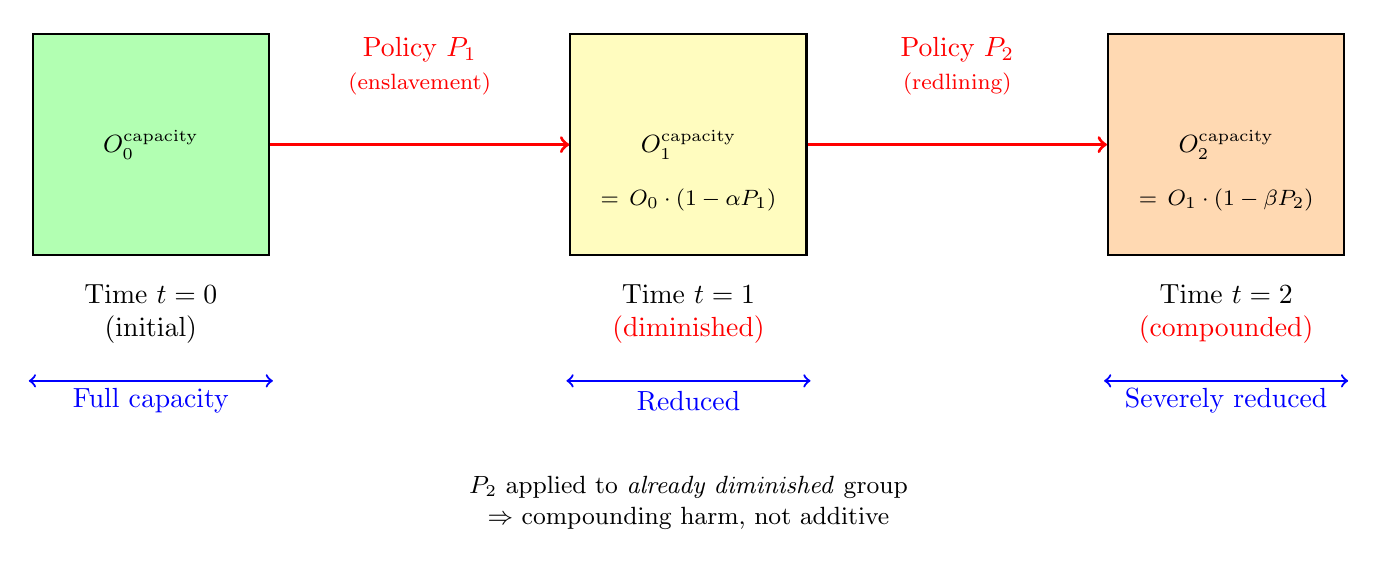
\begin{tikzpicture}[every node/.style={font=\small}]
    % Capacity boxes
    \node[draw, thick, fill=green!30, minimum width=3cm, minimum height=2.8cm] (o0) at (0,0) {$O_0^{\text{capacity}}$};
    \node[draw, thick, fill=yellow!25, minimum width=3cm, minimum height=2.8cm, right=3.8cm of o0] (o1) {$O_1^{\text{capacity}}$};
    \node[draw, thick, fill=orange!30, minimum width=3cm, minimum height=2.8cm, right=3.8cm of o1] (o2) {$O_2^{\text{capacity}}$};

    % Capacity equations
    \node[font=\footnotesize] at ($(o1)+(0,-0.7)$) {$=\, O_0 \cdot (1-\alpha P_1)$};
    \node[font=\footnotesize] at ($(o2)+(0,-0.7)$) {$=\, O_1 \cdot (1-\beta P_2)$};

    % Policy arrows
    \draw[->, very thick, red] (o0.east) -- (o1.west);
    \draw[->, very thick, red] (o1.east) -- (o2.west);
    \node[red, font=\normalsize, align=center] at ($(o0)!0.5!(o1)+(0,1.0)$) {Policy $P_1$\\\footnotesize(enslavement)};
    \node[red, font=\normalsize, align=center] at ($(o1)!0.5!(o2)+(0,1.0)$) {Policy $P_2$\\\footnotesize(redlining)};

    % Time labels
    \node[font=\normalsize] at ($(o0)+(0,-1.9)$) {Time $t=0$};
    \node[font=\normalsize] at ($(o0)+(0,-2.35)$) {(initial)};

    \node[font=\normalsize] at ($(o1)+(0,-1.9)$) {Time $t=1$};
    \node[font=\normalsize, red] at ($(o1)+(0,-2.35)$) {(diminished)};

    \node[font=\normalsize] at ($(o2)+(0,-1.9)$) {Time $t=2$};
    \node[font=\normalsize, red] at ($(o2)+(0,-2.35)$) {(compounded)};

    % Visual representation of shrinking
    \draw[<->, thick, blue] ($(o0)+(-1.55,-3)$) -- ($(o0)+(1.55,-3)$);
    \node[blue, font=\normalsize] at ($(o0)+(0,-3.25)$) {Full capacity};

    \draw[<->, thick, blue] ($(o1)+(-1.55,-3)$) -- ($(o1)+(1.55,-3)$);
    \node[blue, font=\normalsize] at ($(o1)+(0,-3.25)$) {Reduced};

    \draw[<->, thick, blue] ($(o2)+(-1.55,-3)$) -- ($(o2)+(1.55,-3)$);
    \node[blue, font=\normalsize] at ($(o2)+(0,-3.25)$) {Severely reduced};

    % Annotation
    \node[align=center, font=\small] at ($(o1)+(0,-4.55)$) {$P_2$ applied to \textit{already diminished} group\\$\Rightarrow$ compounding harm, not additive};
\end{tikzpicture}
\caption{Temporal compounding model: Each policy reduces Out-group capacity, making subsequent policies more harmful. Policy $P_2$ (redlining) causes greater harm when applied to a group already diminished by $P_1$ (enslavement).}
\label{fig:compounding}
\end{figure}

\begin{figure}[htbp]
\centering
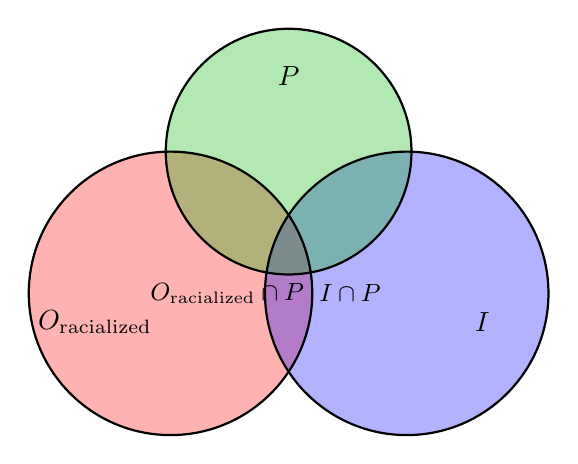
\begin{tikzpicture}[scale=1.2]
    % Define the circles
    \def\circleA{(0,0) circle (1.5cm)}
    \def\circleB{(2.5,0) circle (1.5cm)}
    \def\circleC{(1.25,1.5) circle (1.3cm)}
    
    % Fill the intersections with different shades
    \begin{scope}[fill opacity=0.3]
        \fill[red] \circleA;
        \fill[blue] \circleB;
        \fill[green!70!black] \circleC;
    \end{scope}
    
    % Draw the circles
    \draw[thick] \circleA;
    \draw[thick] \circleB;
    \draw[thick] \circleC;
    
    % Add labels
    \node at (-0.8,-0.3) {$O_{\text{racialized}}$};
    \node at (3.3,-0.3) {$I$};
    \node at (1.25,2.3) {$P$};
    
    % Add description of intersections
    \node[align=center, font=\small] at (0.6,0) {$O_{\text{racialized}} \cap P$};
    \node[align=center, font=\small] at (1.9,0) {$I \cap P$};
\end{tikzpicture}
\caption{Venn diagram illustrating the relationships between the Out-group ($O_{\text{racialized}}$), Policies ($P$), and In-group ($I$), showing how policies intersect differently with each group.}
\label{fig:venn_model}
\end{figure}

\subsection{Historical Policies as Case Studies}

Historical policies, such as the Portuguese slave trade and subsequent colonial practices, serve as real-world examples of our model. These policies created and perpetuated disparities between racial groups, institutionalizing racism at a systemic level.

\subsection{Introducing the Elite Class: A Three-Tier Model}

However, the binary In-group/Out-group model, while useful, obscures a crucial dynamic. A more accurate representation requires introducing a third set: the Elite ($E$), the true beneficiaries of systemic oppression. We can now model society as:
\[
E \subset I, \quad \text{where} \quad |E| \ll |I|
\]
The Elite constitute a small subset of the nominal In-group, yet they are the primary architects and beneficiaries of oppressive policies. The broader In-group ($I \setminus E$)---ordinary members of the dominant racial group---receive psychological and social benefits (what W.E.B.\ Du Bois termed the ``wages of whiteness'') but not the material benefits that accrue to the Elite.

\begin{figure}[htbp]
\centering
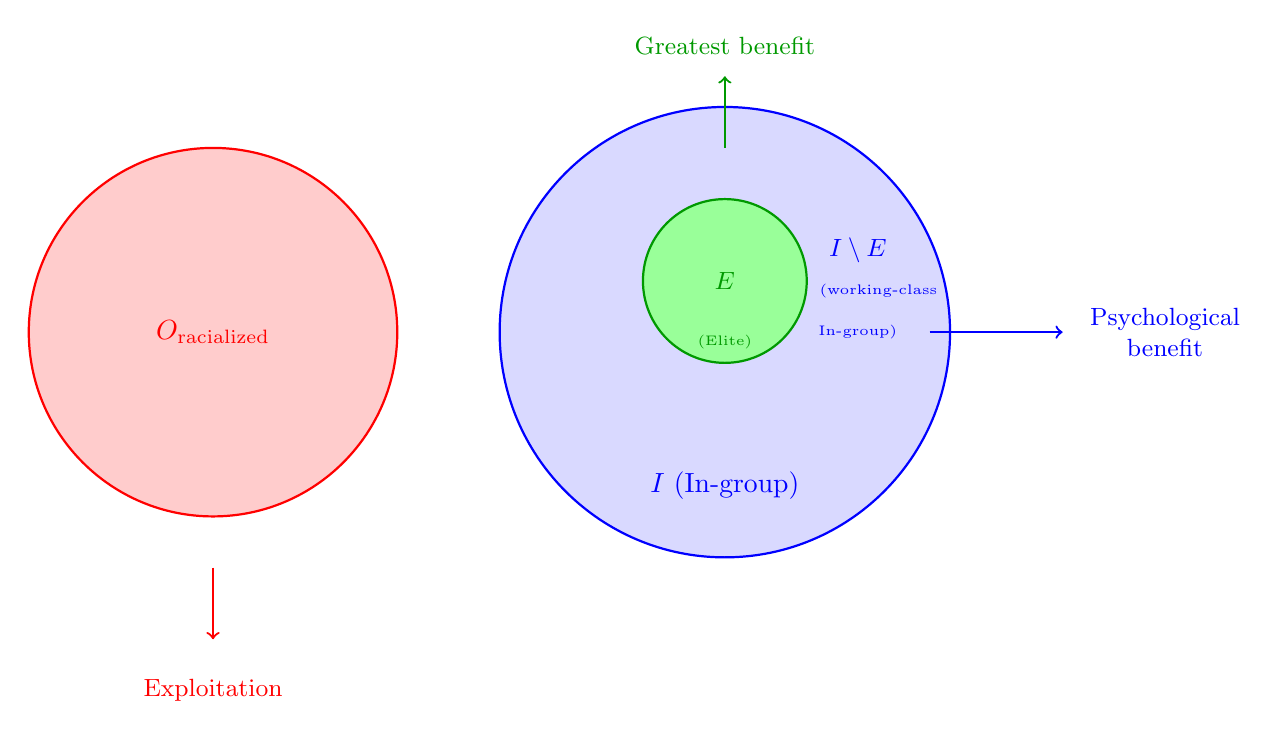
\begin{tikzpicture}[scale=1.3]
    % Draw the Out-group (large circle on left)
    \draw[thick, red, fill=red!20] (-3,0) circle (1.8cm);
    \node[red] at (-3,0) {$O_{\text{racialized}}$};
    
    % Draw the In-group (large circle on right)
    \draw[thick, blue, fill=blue!15] (2,0) circle (2.2cm);
    \node[blue] at (2,-1.5) {$I$ (In-group)};
    
    % Draw the Elite (small circle inside In-group)
    \draw[thick, green!60!black, fill=green!40] (2,0.5) circle (0.8cm);
    \node[green!60!black, font=\small] at (2,0.5) {$E$};
    \node[green!60!black, font=\tiny] at (2,-0.1) {(Elite)};
    
    % Draw the non-Elite In-group region label - moved inside circle, away from boundary
    \node[blue, font=\small] at (3.3,0.8) {$I \setminus E$};
    \node[blue, font=\tiny] at (3.5,0.4) {(working-class};
    \node[blue, font=\tiny] at (3.3,0.0) {In-group)};
    
    % Arrow annotations showing benefit flow
    \draw[->, thick, green!60!black] (2,1.8) -- (2,2.5);
    % "Greatest benefit" moved above arrow
    \node[green!60!black, font=\small] at (2,2.8) {Greatest benefit};
    
    % Psychological benefit arrow - shifted right more
    \draw[->, thick, blue] (4.0,0) -- (5.3,0);
    \node[blue, font=\small, align=center] at (6.3,0) {Psychological\\benefit};
    
    \draw[->, thick, red] (-3,-2.3) -- (-3,-3);
    \node[red, font=\small] at (-3,-3.5) {Exploitation};
\end{tikzpicture}
\caption{Three-tier model showing Elite ($E$) as small subset of In-group ($I$), with Out-group ($O_{\text{racialized}}$) exploited to benefit Elite while $(I \setminus E)$ receives psychological compensation.}
\label{fig:elite_model}
\end{figure}

This leads to a critical insight: the system does not truly serve the In-group; it serves the Elite while using racial division to prevent solidarity between $(I \setminus E)$ and $O_{\text{racialized}}$. Mathematically:
\[
\text{Benefit}(E) \gg \text{Benefit}(I \setminus E) > \text{Benefit}(O_{\text{racialized}})
\]

\section{Policing, Class, and Racial Control: A Set-Theoretic Analysis}

The history of policing in America provides a compelling case study of how systemic racism has been institutionalized and evolved over centuries. Crucially, this history demonstrates an expanding Out-group---revealing that the system of oppression does not ultimately protect the In-group but rather serves to periodically reset and expand the subjugated class whenever necessary to maintain Elite control.

Let us define the Out-group at any time $t$ as $O_t$, and trace its expansion through American history.

\subsection{Origins: Slave Patrols (Early 1700s)}

The first form of organized policing in the American colonies originated in the South as slave patrols. These patrols were explicitly designed to preserve the institution of slavery by capturing escaped enslaved people and suppressing potential rebellions.

At this stage, we can define:
\[
O_{1700} = \{\text{Enslaved Africans}\}
\]
The Out-group was explicitly racial, and the nominal In-group included all free persons. However, even here, the Elite ($E$)---slaveholding planters---were the true beneficiaries. Poor whites were recruited into slave patrols, receiving minimal compensation but psychological investment in racial hierarchy. This arrangement prevented class solidarity between poor whites and enslaved Blacks, a deliberate strategy following events like Bacon's Rebellion (1676), where poor whites and Blacks had united against the colonial elite.

\subsection{Formalization of Police Forces (1830s--1860s)}

The establishment of the Boston Police Department in the 1830s marked the creation of the first modern police department in the United States. While publicly funded by all taxpayers, these early departments primarily served to protect the property and interests of the Elite.

The Fugitive Slave Act of 1850 is particularly revealing. By April 24, 1851, Boston police---in a Northern ``free'' state---were actively assisting in the capture and return of escaped slaves. This demonstrates:
\[
P_{\text{Fugitive Slave Act}} \cap (I \setminus E) \neq \emptyset
\]
Northern workers, nominally part of the In-group, were compelled to participate in slave-catching, and those who refused faced penalties. The system began demanding active complicity from the broader In-group while offering them no material benefit.

\subsection{Constitutional Exclusion: Dred Scott (1857)}

Before the Civil War, the Supreme Court explicitly addressed the question of who constitutes ``the people'' with constitutional rights. In \textit{Dred Scott v. Sandford} (1857), Chief Justice Taney excluded Black people from ``the people,'' declaring they ``had no rights which the white man was bound to respect.'' Taney's reasoning was revealing: if Black people were included among ``the people,'' they would have the right to keep and bear arms---an outcome he found unacceptable.

This established a constitutional mechanism for defining the Out-group:
\[
O_{1857} = \{\text{Enslaved Africans}\} \cup \{\text{Free Blacks}\}
\]
The phrase ``the people'' appears throughout the Constitution---in the First, Second, Fourth, and Fourteenth Amendments---and serves as the hinge upon which rights turn. \textit{Dred Scott} made explicit that this phrase could be narrowed to exclude entire categories of persons, making their rights conditional rather than inherent.

\subsection{The 13th Amendment and Its Loophole (1865)}

The 13th Amendment abolished slavery ``except as punishment for a crime.'' This exception represents the first major \textbf{expansion} of the Out-group through a new mechanism:
\[
O_{1865} = \{\text{Black Americans}\} \cup \{\text{Convicts}\}
\]
Since $\{\text{Black Americans}\} \cap \{\text{Convicts}\}$ was maximized through the Black Codes---laws specifically designed to criminalize Black behavior---the primary targets remained Black Americans. However, the theoretical framework now permitted \textit{any} person convicted of a crime to be subjected to slavery.

Through convict leasing and chain gangs, the criminal justice system became a mechanism for maintaining a racialized labor underclass. The Elite gained access to cheap convict labor, while poor whites were told their freedom depended on maintaining racial hierarchy---even as they themselves became increasingly vulnerable to the expanding carceral state.

The 13th Amendment's ``except as punishment for a crime'' clause provided a template: define conduct as criminal, then strip constitutional rights from those convicted. After the 13th, 14th, and 15th Amendments made explicit racial exclusion unconstitutional, ``criminals'' and ``felons'' became the new proxy for racial exclusion.

\subsection{Jim Crow Era Enforcement (1900--1965)}

During the Jim Crow era, police served as the enforcement arm of segregation laws. The Out-group remained:
\[
O_{\text{Jim Crow}} = \{\text{Black Americans}\} \cup \{\text{Convicts}\}
\]
However, the system required increasing participation from the broader In-group. Poor whites were recruited as enforcers of segregation---as Klansmen, as participants in lynch mobs, as voters for segregationist politicians. The psychological wages of whiteness substituted for material advancement, while the Elite accumulated wealth from a segregated labor market that suppressed wages for \textit{all} workers.

The constitutional exclusion mechanism was refined during this period through grandfather clauses, literacy tests, and property requirements that maintained white privilege while excluding Black Americans from voting, jury service, and gun ownership---all rights of ``the people.'' These facially neutral restrictions created a model for future exclusions that could operate without explicit racial language.

\subsection{Civil Rights Advances (1954--1965): A Temporary Contraction}

The period from 1954 to 1965 brought significant legal victories against institutionalized racism. \textit{Brown v.\ Board of Education} (1954) ended ``separate but equal'' segregation. The Civil Rights Act (1964) and Voting Rights Act (1965) dismantled the legal framework of Jim Crow.

This period represents a temporary \textbf{contraction} of the explicit Out-group:
\[
O_{1965} \xrightarrow{\text{legal changes}} O'_{1965}, \quad |O'_{1965}| < |O_{1965}|
\]
Explicitly racialized laws became unconstitutional. However, this contraction threatened Elite interests by potentially enabling cross-racial class solidarity. The response was swift.

\subsection{The Counterattack: Southern Strategy and Economic Targeting (Late 20th Century)}

Following civil rights victories, new strategies emerged to maintain racial hierarchies without explicit racial language. Lee Atwater's ``Southern Strategy'' employed coded language to continue the criminalization of Blackness through ostensibly race-neutral policies.

\textbf{The Abstraction of Racism Back Into Economics: Completing the Circle}

What Lee Atwater accomplished was profound: he \textbf{abstracted racism back into economics}, returning the system to its foundational logic as a tool of class oppression. This was not the elimination of racism but its \textit{refinement}---racism still operated, but now it functioned primarily through \textbf{economic class undertones}, returning to its roots as a mechanism for maintaining a slave class.

Atwater's famous 1981 interview makes this explicit:

\begin{quote}
``You start out in 1954 by saying, `N*****, n*****, n*****.' By 1968 you can't say `n*****'---that hurts you, backfires. So you say stuff like, uh, forced busing, states' rights, and all that stuff, and you're getting so abstract. Now, you're talking about cutting taxes, and all these things you're talking about are totally economic things and a byproduct of them is, blacks get hurt worse than whites... `We want to cut this,' is much more abstract than even the busing thing, uh, and a hell of a lot more abstract than `N*****, n*****.'``
\end{quote}

This reveals the strategic evolution:

\begin{enumerate}
    \item \textbf{Stage 1 (Pre-Civil Rights)}: Explicit racial language---overt racism maintaining the slave class
    \item \textbf{Stage 2 (Post-Civil Rights)}: Coded racial language---``states' rights,'' ``forced busing''
    \item \textbf{Stage 3 (Atwater's Innovation)}: Economic abstraction---tax cuts, welfare reform, ``entitlement'' reduction
\end{enumerate}

\textbf{By Stage 3, racism had been abstracted into economics so thoroughly that it became indistinguishable from class warfare}. But crucially, it remained racism---because the policies were designed to harm Black Americans disproportionately while \textit{simultaneously} expanding the subjugated class to include poor whites. This was the Elite's endgame all along: return to a pure class hierarchy where race is used to prevent solidarity among the exploited.

\textbf{Expanding the Slave Class: Always the Goal}

Crucially, these policies began \textbf{expanding} the Out-group to include poor whites:
\[
O_{1980} = \{\text{Black Americans}\} \cup \{\text{Convicts}\} \cup \{\text{The Poor}\}
\]
Redlining and discriminatory economic policies systematically targeted Black communities, creating concentrated poverty. But deindustrialization, union-busting, and neoliberal economic policies simultaneously devastated white working-class communities. The Elite were consolidating wealth while \textit{both} racial groups experienced declining economic mobility.

This was not a failure of the system---it was the \textit{point}. The Elite never intended to maintain white working-class prosperity; they needed racial hierarchy to:
\begin{itemize}
    \item \textbf{Prevent solidarity during the expansion}: Keep poor whites blaming poor Blacks while both groups are immiserated
    \item \textbf{Test economic policies on racialized groups first}: Policies designed to harm Black Americans (welfare reform, public housing destruction, deinvestment in education) could then be expanded to white communities under economic justifications
    \item \textbf{Return to slave capitalism's core logic}: Maintain an exploitable underclass unconstrained by moral limits, now rationalized through economic ``efficiency'' rather than racial inferiority
\end{itemize}

The genius of the Southern Strategy was not just convincing poor whites that their enemies were Black Americans and ``welfare queens'' rather than the Elite extracting wealth from both groups. It was \textbf{abstracting racism into economic policy that could expand the slave class across racial lines while maintaining racial division to prevent resistance}.

\textbf{The Return to Foundational Class Logic}

By abstracting racism into economics, Atwater's strategy brought the system full circle back to its 15th-century Portuguese origins:

\begin{itemize}
    \item \textbf{Then}: Elite needed exploitable labor, invented race to create slave class while preventing working-class solidarity
    \item \textbf{Now}: Elite need exploitable labor, use economic policy (abstracted racism) to expand subjugated class while preventing working-class solidarity
\end{itemize}

The difference is sophistication: modern slave capitalism doesn't require explicit racial categorization because economic policies racialized through coded language achieve the same function. The slave class expands ``race-neutrally'' through policies that disproportionately harm Black Americans first, then spread to poor whites, all while appearing to be about ``fiscal responsibility'' or ``economic efficiency.''

This is the expansion of the slave class---which was always the Elite's goal from the beginning of slave capitalism. Racism was invented to create and maintain a subjugated class; it is now being abstracted back into economics to \textit{expand} that class while retaining racial division as the mechanism that prevents unified resistance.

\subsection{War on Drugs and Mass Incarceration (1980s--1990s)}

The War on Drugs represented a dramatic expansion of the Out-group:
\[
O_{1990} = \{\text{Black Americans}\} \cup \{\text{Convicts}\} \cup \{\text{The Poor}\} \cup \{\text{Drug Users}\}
\]
The introduction of crack cocaine into Black neighborhoods, combined with harsh sentencing disparities (100:1 crack vs. powder cocaine), created conditions for mass incarceration that disproportionately affected Black communities. But the War on Drugs also ensnared millions of white Americans.

\begin{quote}
``The Nixon campaign in 1968, and the Nixon White House after that, had two enemies: the antiwar left and black people.''

\emph{(Paraphrase of the remainder of the statement)} Ehrlichman then explains that, while they could not criminalize being antiwar or Black, they associated hippies with marijuana and Black people with heroin and then heavily criminalized both to disrupt those communities and arrest their leaders, concluding: ``Did we know we were lying about the drugs? Of course we did.'' (as quoted in Baum, 2016)\cite{baum}
\end{quote}

\textbf{The United States as Prison Capital of the World}

By the 1990s, the United States had achieved a jarring distinction: \textbf{the highest incarceration rate in the world}. The statistics reveal an anomaly of staggering proportions:

\begin{itemize}
    \item \textbf{Scale}: The U.S. holds approximately 2.3 million people in prisons and jails (as of 2020s)
    \item \textbf{Rate}: With roughly 4\% of the world's population, the U.S. holds nearly 25\% of the world's prisoners
    \item \textbf{Incarceration rate}: Approximately 700 per 100,000 people---5-10 times higher than most other democracies
    \item \textbf{Growth}: Prison population increased by over 500\% between 1970 and 2000, far outpacing crime rates
    \item \textbf{Comparison}: U.S. incarceration rate exceeds authoritarian regimes and every Western democracy by multiples
\end{itemize}

\textbf{Racial Composition: The 13th Amendment's Legacy}

The racial makeup of U.S. prisons exposes the continuity with slave capitalism:

\begin{itemize}
    \item \textbf{Black Americans}: Comprise approximately 13\% of U.S. population but 38\% of prison population
    \item \textbf{Incarceration disparity}: Black men are incarcerated at 5-6 times the rate of white men
    \item \textbf{Lifetime likelihood}: 1 in 3 Black men born today can expect to be imprisoned at some point, compared to 1 in 17 white men
    \item \textbf{Hispanic Americans}: Comprise 18\% of population but 21\% of prison population
    \item \textbf{Drug offenses}: Despite similar usage rates across races, Black Americans are arrested for drug offenses at 2-3 times the rate of white Americans
\end{itemize}

These disparities are not accidental---they represent the successful operation of the 13th Amendment's ``except as punishment for a crime'' loophole, creating a racialized carceral system that mirrors slavery's demographics.

\textbf{The Prison-Industrial Complex: Slave Capitalism Modernized}

The prison-industrial complex represents the evolution of slave capitalism into a multi-billion dollar industry:

\begin{itemize}
    \item \textbf{For-profit prisons}: Corporations like CoreCivic (formerly Corrections Corporation of America) and GEO Group profit directly from incarceration, creating financial incentives to expand the imprisoned population
    \item \textbf{Prison labor}: Incarcerated people work for pennies per hour (often \$0.14-\$0.63/hour, sometimes nothing), producing goods and services while corporations profit---modern slavery under the 13th Amendment exception
    \item \textbf{Contractual quotas}: Some private prison contracts include ``lockup quotas'' requiring states to maintain 90-100\% occupancy or pay penalties, creating perverse incentives to incarcerate
    \item \textbf{Ancillary industries}: Phone companies, commissary suppliers, bail bond companies, electronic monitoring firms---entire industries profit from the carceral system
    \item \textbf{Financial sector}: Wall Street banks finance prison construction; investors profit from prison bonds and stocks
    \item \textbf{Political influence}: Prison corporations donate to political campaigns and lobby for harsher sentencing laws, creating a feedback loop that expands their market
\end{itemize}

\textbf{The School-to-Prison Pipeline: Manufacturing the Slave Class}

The expansion of the carceral system required a mechanism to continuously supply prisoners. The school-to-prison pipeline serves this function:

\begin{itemize}
    \item \textbf{Zero-tolerance policies}: Beginning in 1990s, schools adopted policies that criminalize normal childhood behavior, particularly in predominantly Black and Hispanic schools
    \item \textbf{Police in schools}: School Resource Officers arrest students for minor infractions that were once handled by principals, introducing children to the criminal justice system
    \item \textbf{Disparate discipline}: Black students are 3-4 times more likely to be suspended or expelled than white students for the same behavior
    \item \textbf{Special education to prison}: Students with disabilities are disproportionately funneled into the criminal justice system through school discipline
    \item \textbf{Funding disparities}: Schools in predominantly Black neighborhoods receive less funding, have fewer resources, and higher police presence---creating conditions for failure and criminalization
    \item \textbf{Early tracking}: Students identified as ``problems'' in elementary school are tracked toward incarceration rather than education
\end{itemize}

This pipeline manufactures the future prison population by criminalizing children in Black and poor communities, ensuring a steady supply of bodies for the prison-industrial complex. It is the modern equivalent of breeding enslaved people to maintain the slave population---except now it operates through policy rather than biology.

The expansion of what constitutes ``crime'' during this period directly expanded the Out-group. The definition of criminal conduct broadened to encompass drug possession, low-level offenses, and behaviors that had previously been legal or subject to minimal penalties. This expansion operated through the constitutional mechanism established in \textit{Dred Scott} and refined through the 13th Amendment: define conduct as criminal, then strip rights from those convicted.

\textbf{The Elite Benefit: Following the Money}

Who profits from mass incarceration?

\begin{itemize}
    \item \textbf{Private prison corporations}: Multi-billion dollar industry with guaranteed revenue
    \item \textbf{Prison labor contractors}: Access to captive workforce at below-minimum wage
    \item \textbf{Financial institutions}: Profit from financing prison construction and operations
    \item \textbf{Ancillary service providers}: Phone companies charging \$1-5 per minute for prison calls; commissary suppliers marking up goods 200-300\%
    \item \textbf{Political campaigns}: Prison corporations and unions contribute to politicians who support tough-on-crime policies
    \item \textbf{Rural communities}: Prisons bring jobs and federal funding (prisoners counted for Census but can't vote)
\end{itemize}

Meanwhile, the imprisoned---disproportionately Black and poor---provide the labor, pay the fees, and lose their rights. The prison-industrial complex is slave capitalism with a corporate structure, and the Out-group continues to expand to meet demand.

\subsection{Rights Erosion and Modern Exclusion (1970s--Present)}

The expansion of the Out-group accelerated through incremental erosion of rights themselves. The definition of ``crime'' expanded to encompass ever more conduct, and millions of Americans became excluded from ``the people'' through felony disenfranchisement, firearms prohibitions, and civil disabilities that follow criminal conviction.

Each restriction creates a new category of excluded persons:

\begin{itemize}
    \item \textbf{Temporal Classifications}: Laws that ``grandfather'' existing rights-holders while prohibiting new ones create tiered citizenship. Those who owned certain items before a cutoff date retain rights; those who seek to acquire them after do not.
    \item \textbf{Economic Barriers}: Poll taxes, fees, and compliance costs exclude those without economic resources. When rights require payment to exercise, poverty becomes disqualifying.
    \item \textbf{Administrative Burdens}: Licensing requirements, waiting periods, and bureaucratic processes exclude those without time, transportation, or knowledge to navigate systems.
    \item \textbf{Age Restrictions}: Raising age thresholds for rights (voting, firearms, alcohol) expands the period during which citizens are excluded from ``the people.''
\end{itemize}

Each mechanism adds members to the Out-group without explicitly naming them:
\[
O_{\text{present}} = O_{1990} \cup \{\text{Felons}\} \cup \{\text{The Poor}\} \cup \{\text{The Young}\} \cup \{\text{The Administratively Excluded}\}
\]

\textbf{The Current Reality: Mass Incarceration and the Modern Slave Class}

The United States maintains its status as the \textbf{prison capital of the world}---a distinction that represents the successful expansion of the Out-group through the carceral system:

\begin{itemize}
    \item \textbf{Felony convictions}: Approximately 19 million Americans have felony convictions
    \item \textbf{Criminal records}: An additional 77 million have some form of criminal record (nearly 1 in 3 American adults)
    \item \textbf{Current incarceration}: 2.3 million people currently imprisoned
    \item \textbf{Correctional control}: Over 6.5 million people under some form of correctional supervision (prison, jail, parole, probation)
    \item \textbf{Global anomaly}: With 4\% of world population, U.S. holds 25\% of world's prisoners---an incarceration rate of ~700 per 100,000, compared to ~100 per 100,000 in most Western democracies
\end{itemize}

These individuals face varying degrees of exclusion from ``the people'':

\begin{itemize}
    \item \textbf{Disenfranchisement}: 5.2 million Americans denied voting rights due to felony convictions (disproportionately Black: 1 in 13 Black Americans vs. 1 in 56 non-Black Americans)
    \item \textbf{Employment discrimination}: Criminal records create permanent barriers to employment, even decades after release
    \item \textbf{Housing exclusion}: Public housing bans and private landlord discrimination based on criminal history
    \item \textbf{Firearms prohibitions}: Federal law strips gun rights from anyone with a felony conviction
    \item \textbf{Educational barriers}: Limited access to financial aid, professional licenses, and educational opportunities
    \item \textbf{Family separation}: Children of incarcerated parents face increased risk of poverty, homelessness, and future incarceration
\end{itemize}

\textbf{The Racial Reality}

The carceral state has created a permanent underclass that crosses racial lines while still disproportionately affecting Black Americans:

\begin{itemize}
    \item \textbf{Black men}: 1 in 3 will be imprisoned at some point in their lives
    \item \textbf{Black women}: Fastest-growing incarcerated demographic, often crimi\-nalized for poverty-related offenses
    \item \textbf{Generational impact}: Children of incarcerated parents are 6 times more likely to be incarcerated themselves
    \item \textbf{Community devastation}: Some predominantly Black neighborhoods have incar\-ceration rates above 50\% for working-age men
    \item \textbf{Economic extraction}: Families pay billions annually in fees, phone calls, commissary markups, and bail---transferring wealth from poor Black communities to corporations
\end{itemize}

Yet the expansion continues beyond racial lines: poor white communities now face similar criminalization, opioid-related prosecutions, and carceral control. The slave class expands, fulfilling the Elite's original goal while maintaining racial division to prevent solidarity.

This mechanism reveals the expansion's logic: the system no longer needs to explicitly name racial groups when it can define behaviors associated with marginalized communities as criminal, then strip rights from anyone so labeled. The Out-group expands through the ever-broadening definition of ``dangerous'' rather than through explicit racial categorization. The 13th Amendment's ``except as punishment for crime'' clause provides the constitutional mechanism; the prison-industrial complex provides the economic incentive; and the school-to-prison pipeline provides the supply chain for modern slave capitalism.

\textbf{The Slippery Slope as Documented Pattern}

The ``slippery slope'' is often dismissed as a logical fallacy. But there is a crucial distinction between an unfounded prediction and a documented historical pattern. The expansion of the Out-group through incremental restrictions is not speculation---it is the observable trajectory of American history:

\begin{enumerate}
    \item Rights once held by ``the whole people'' are restricted to subsets
    \item Restrictions expand through administrative, economic, and temporal mechanisms
    \item Each restriction creates precedent for further restriction
    \item The definition of ``dangerous'' or ``unqualified'' broadens
    \item More of the population falls outside ``the people''
\end{enumerate}

This pattern explains why the Out-group expands even when explicit discrimination is prohibited: the system continuously generates new categories of exclusion.

\subsection{The Expanding Out-Group: Mathematical Formalization}

We can now formalize the expansion of the Out-group over time:
\[
O_{1700} \subset O_{1857} \subset O_{1865} \subset O_{\text{Jim Crow}} \subset O_{1980} \subset O_{1990} \subset O_{\text{present}}
\]
Each inclusion is proper: the Out-group strictly expands. This expansion reveals a fundamental truth: \textbf{the system of racial oppression does not protect the In-group; it gradually consumes it}.

\begin{figure}[htbp]
\centering
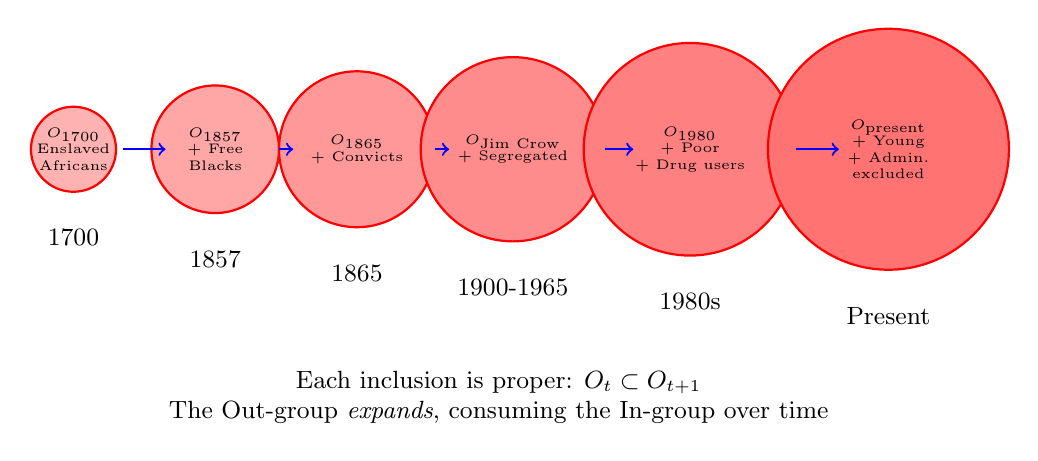
\begin{tikzpicture}[scale=0.9]
    % 1700 - smallest circle
    \draw[thick, red, fill=red!30] (0,0) circle (0.6cm);
    \node[font=\tiny, align=center] at (0,0) {$O_{1700}$\\Enslaved\\Africans};
    \node[font=\small, below] at (0,-1) {1700};
    
    % 1857 - Dred Scott
    \draw[thick, red, fill=red!35] (2,0) circle (0.9cm);
    \node[font=\tiny, align=center] at (2,0) {$O_{1857}$\\+ Free\\Blacks};
    \node[font=\small, below] at (2,-1.3) {1857};
    
    % 1865 - 13th Amendment
    \draw[thick, red, fill=red!40] (4,0) circle (1.1cm);
    \node[font=\tiny, align=center] at (4,0) {$O_{1865}$\\+ Convicts};
    \node[font=\small, below] at (4,-1.5) {1865};
    
    % Jim Crow
    \draw[thick, red, fill=red!45] (6.2,0) circle (1.3cm);
    \node[font=\tiny, align=center] at (6.2,0) {$O_{\text{Jim Crow}}$\\+ Segregated};
    \node[font=\small, below] at (6.2,-1.7) {1900-1965};
    
    % 1980s - Southern Strategy
    \draw[thick, red, fill=red!50] (8.7,0) circle (1.5cm);
    \node[font=\tiny, align=center] at (8.7,0) {$O_{1980}$\\+ Poor\\+ Drug users};
    \node[font=\small, below] at (8.7,-1.9) {1980s};
    
    % Present
    \draw[thick, red, fill=red!55] (11.5,0) circle (1.7cm);
    \node[font=\tiny, align=center] at (11.5,0) {$O_{\text{present}}$\\+ Young\\+ Admin.\\excluded};
    \node[font=\small, below] at (11.5,-2.1) {Present};
    
    % Arrows showing expansion
    \draw[->, thick, blue] (0.7,0) -- (1.3,0);
    \draw[->, thick, blue] (2.9,0) -- (3.1,0);
    \draw[->, thick, blue] (5.1,0) -- (5.3,0);
    \draw[->, thick, blue] (7.5,0) -- (7.9,0);
    \draw[->, thick, blue] (10.2,0) -- (10.8,0);
    
    % Annotation
    \node[align=center, font=\small] at (6,-3.5) {Each inclusion is proper: $O_{t} \subset O_{t+1}$\\The Out-group \textit{expands}, consuming the In-group over time};
\end{tikzpicture}
\caption{The expanding Out-group over time. Each circle represents a proper superset of the previous, showing how the Out-group grows to encompass groups once part of the In-group.}
\label{fig:expanding_outgroup}
\end{figure}

Let us define the ``Slave Class'' $S_t$ at time $t$ as those subject to unfree labor or severe economic exploitation:
\[
|S_t| \xrightarrow{t \to \text{present}} \text{increasing}
\]
The percentage of Americans subject to carceral control, poverty wages, debt bondage, and economic precarity has \textit{increased} over time---even as explicit racial barriers were removed.

\subsection{The Fundamental Inequality}

This analysis reveals that the core inequality is not between In-group and Out-group but between Elite and everyone else:
\[
\text{Benefit}(E) \gg \text{Benefit}(I \cup O_{\text{racialized}} \setminus E)
\]
Racial division serves to prevent the recognition of this fundamental inequality. As the Out-group expands to encompass more of the former In-group, we approach a return to pre-racial class structures---but with the added tool of racial division to prevent unified resistance.

\begin{figure}[htbp]
\centering
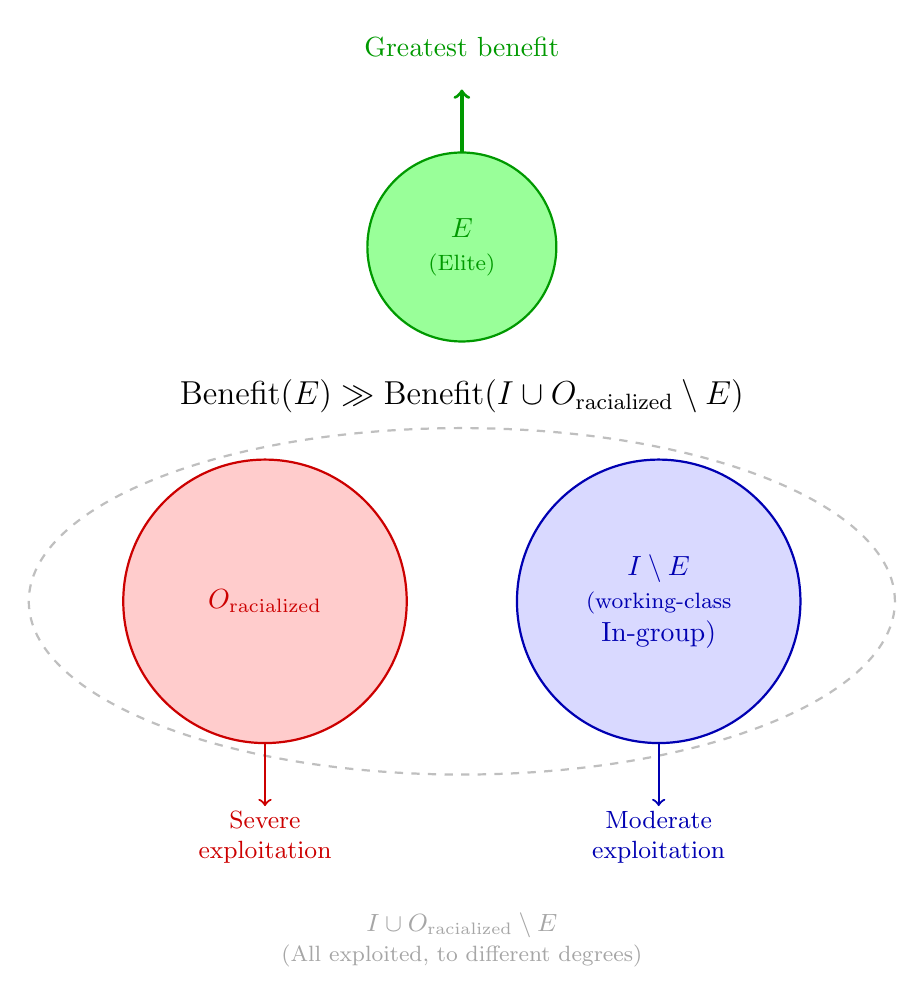
\begin{tikzpicture}[scale=1.0]
    % Elite circle at top - separate and emphasized
    \draw[thick, green!60!black, fill=green!40] (0,3) circle (1.2cm);
    \node[green!60!black, font=\normalsize, align=center] at (0,3) {$E$\\\footnotesize(Elite)};
    
    % Arrow showing Elite benefit
    \draw[->, very thick, green!60!black] (0,4.2) -- (0,5.0);
    \node[green!60!black, font=\normalsize, above] at (0,5.3) {Greatest benefit};
    
    % Unified exploited group at bottom - showing both I\E and O together
    % Out-group on left
    \draw[thick, red!80!black, fill=red!20] (-2.5,-1.5) circle (1.8cm);
    \node[red!80!black, font=\normalsize, align=center] at (-2.5,-1.5) {$O_{\text{racialized}}$};
    
    % Working-class In-group on right
    \draw[thick, blue!70!black, fill=blue!15] (2.5,-1.5) circle (1.8cm);
    \node[blue!70!black, font=\normalsize, align=center] at (2.5,-1.5) {$I \setminus E$\\\footnotesize(working-class\\In-group)};
    
    % Dashed ellipse showing the unified exploited group
    \draw[thick, dashed, gray!50] (0,-1.5) ellipse (5.5cm and 2.2cm);
    \node[gray!70, font=\small, align=center] at (0,-5.8) {$I \cup O_{\text{racialized}} \setminus E$\\\footnotesize(All exploited, to different degrees)};
    
    % Exploitation arrows
    \draw[->, thick, red!80!black] (-2.5,-3.3) -- (-2.5,-4.1);
    \node[red!80!black, font=\small, align=center] at (-2.5,-4.5) {Severe\\exploitation};
    
    \draw[->, thick, blue!70!black] (2.5,-3.3) -- (2.5,-4.1);
    \node[blue!70!black, font=\small, align=center] at (2.5,-4.5) {Moderate\\exploitation};
    
    % Inequality notation
    \node[font=\large, align=center] at (0,1.1) {$\text{Benefit}(E) \gg \text{Benefit}(I \cup O_{\text{racialized}} \setminus E)$};
\end{tikzpicture}
\caption{Fundamental inequality: Elite ($E$) capture the greatest benefit while the working-class In-group $(I \setminus E)$ receive psychological compensation, and $O_{\text{racialized}}$ bears exploitation.}
\label{fig:fundamental_inequality}
\end{figure}

\subsection{Historical Parallel: Bacon's Rebellion and the Invention of Race}

This dynamic echoes the origins of American racial categorization. Before Bacon's Rebellion (1676), poor Europeans and Africans in Virginia worked side by side under similar conditions of servitude, and they rebelled together against the colonial Elite. In response, the Elite invented rigid racial categories, granting poor whites nominal privileges over Blacks while extracting labor from both.

The current trajectory suggests a ``resetting'' of this arrangement. As economic inequality reaches levels not seen since the Gilded Age, and as the Out-group expands to include more white Americans, we observe:
\begin{enumerate}
    \item Intensified racial rhetoric to maintain division
    \item Expansion of carceral and surveillance systems
    \item Erosion of labor protections affecting all workers
    \item Concentration of wealth among an ever-smaller Elite
\end{enumerate}

The system requires a subjugated class. When that class threatens to shrink (as during civil rights advances), it must be expanded. The question is not \textit{whether} there will be an Out-group but \textit{who} will be consigned to it.

\section{Real-World Applications of the Mathematical Model}

The theoretical framework provided by set theory offers a powerful tool for analyzing systemic racism. To illustrate its practical application, we examine historical examples that highlight the systemic nature of racism, specifically focusing on the Southern Strategy and the practice of redlining in the United States.

\subsection{The Southern Strategy}

The Southern Strategy, employed by the Republican Party under the guidance of strategist Lee Atwater, serves as a poignant example of systemic racism's mechanics. This political strategy was designed to gain support among white voters in the American South by exploiting racial tensions and appealing to anti-Black racism. By utilizing racially coded language and policies, the strategy aimed to subtly but effectively mobilize white voters by capitalizing on existing racial prejudices.

In our mathematical model, we can represent the impact of such a strategy by considering two sets: $B$, the set of all Black individuals, and $W$, the set of all White individuals.

The Southern Strategy's policies and rhetoric predominantly benefited the $W$ set while adversely affecting the $B$ set, creating a stark disparity in political power and social capital. Thus we can model this as:
\[
\sum (B \cap P) \gg \sum (W \cap P)
\]
This means that the sum of policies that adversely impacted the Black community was much higher than the sum of policies that adversely impacted the White community.

\subsection{Redlining}

Redlining represents a more overt form of systemic racism, where services (such as banking, insurance, and access to quality education and healthcare) were systematically denied to residents in predominantly Black neighborhoods. This practice, sanctioned by government agencies and private sectors alike, entrenched socio-economic disparities along racial lines.

Using the mathematical framework, we can model redlining as follows:
\[
B \cap \text{Redlining} \gg W \cap \text{Redlining}
\]
This inequality demonstrates that the policy of redlining disproportionately impacted Black communities ($B$) compared to White communities ($W$), reinforcing a system of racial inequality. Visually, through the lens of modified Venn diagrams, the overlap between the redlining policy and the $B$ set is significantly larger than that of the $W$ set, illustrating the targeted nature of this systemic oppression.

\begin{figure}[htbp]
\centering
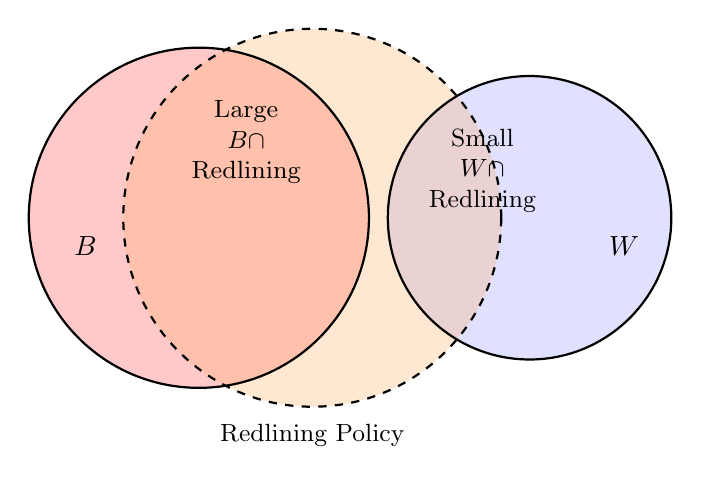
\begin{tikzpicture}[scale=1.2]
    % Define the circles for B, W, and Redlining
    \def\circleB{(0,0) circle (1.8cm)}
    \def\circleW{(3.5,0) circle (1.5cm)}
    \def\circleRedlining{(1.2,0) circle (2cm)}
    
    % Fill the intersections with different shades
    \begin{scope}[fill opacity=0.3]
        \fill[red!70] \circleB;
        \fill[blue!40] \circleW;
        \fill[orange!60] \circleRedlining;
    \end{scope}
    
    % Draw the circles
    \draw[thick] \circleB;
    \draw[thick] \circleW;
    \draw[thick, dashed] \circleRedlining;
    
    % Add labels
    \node at (-1.2,-0.3) {$B$};
    \node at (4.5,-0.3) {$W$};
    \node[font=\small] at (1.2,-2.3) {Redlining Policy};
    
    % Highlight the asymmetric intersection sizes
    \node[align=center, font=\small, text width=2cm] at (0.5,0.8) {Large\\$B \cap$\\Redlining};
    \node[align=center, font=\small] at (3,0.5) {Small\\$W \cap$\\Redlining};
\end{tikzpicture}
\caption{Venn diagram showing the disproportionate impact of redlining policies on Black communities ($B$) versus White communities ($W$), with the intersection $B \cap \text{Redlining}$ being significantly larger than $W \cap \text{Redlining}$.}
\label{fig:redlining_venn}
\end{figure}

\subsection{Implications of the Model}

These real-world examples underscore the utility of our mathematical model in dissecting the systemic nature of racism. Policies like the Southern Strategy and redlining are not anomalies but rather components of a broader system that perpetuates racial inequalities. By applying set theory and discrete mathematics, we can quantitatively and visually represent the impacts of such policies, offering a clearer understanding of systemic racism's dynamics.

These examples highlight the importance of a comprehensive contextual analysis. Understanding the full scope of systemic racism requires examining the cumulative effects of multiple policies over time, as well as their interactions within the broader socio-political landscape. This analytical approach can inform more effective strategies for dismantling systemic racism, guiding policymakers, activists, and communities in their efforts to address racial inequalities at their roots.

\subsection{Policy Implications: Individual vs. Systemic Interventions}

The mathematical framework developed here does not merely describe racism---it \textit{prescribes} specific interventions by revealing where harm is concentrated and how it operates. This framework forces a fundamental shift from individual-focused solutions to systemic policy reform.

\textbf{The Failure of Individual-Focused Solutions}

Traditional approaches to addressing racism often focus on individual prejudice and bias. In the case of lending disparities, for example, this approach leads to interventions such as:
\begin{itemize}
    \item Sensitivity training for loan officers
    \item Implicit bias workshops
    \item Diversity hiring initiatives
    \item Individual complaint mechanisms
\end{itemize}

While these interventions may address individual instances of discrimination, our mathematical model reveals why they cannot address systemic racism. The model identifies the \textit{intersection} $O_{\text{racialized}} \cap P$ as the site of greatest harm. Individual-focused solutions attempt to modify the behavior of actors \textit{within} the system while leaving the policy $P$ unchanged. Mathematically, this is attempting to reduce harm while keeping the structural inequality intact.

Moreover, our temporal compounding model demonstrates that individual bias is \textit{downstream} of systemic design. The accumulated disadvantage represented by $O_t^{\text{capacity}}$ creates disparities that appear even when individual actors have no conscious bias. A loan officer applying ostensibly neutral criteria to applicants with dramatically different accumulated capital (due to historical policies like redlining, employment discrimination, and wealth extraction) will produce racially disparate outcomes even with zero individual prejudice.

\textbf{Systemic Interventions Mandated by the Framework}

Our framework compels a fundamentally different approach. By identifying $O_{\text{racialized}} \cap P$ as the mathematical site of harm, the framework mandates direct intervention on the \textit{policy} $P$ itself:

\textbf{Case Study: Lending Disparities}

The framework demands an audit of the institutional rules and underwriting criteria that constitute $P$. Specific interventions include:
\begin{enumerate}
    \item \textbf{Audit the policy structure}: Examine whether underwriting criteria (credit score thresholds, debt-to-income ratios, down payment requirements, employment history requirements) structurally disadvantage groups with diminished $O_t^{\text{capacity}}$ due to historical policies.
    
    \item \textbf{Measure the intersection}: Quantify $|O_{\text{racialized}} \cap P_{\text{current}}|$---the number of Out-group members adversely affected by current policy---and compare to $|I \cap P_{\text{current}}|$.
    
    \item \textbf{Redesign policy parameters}: Modify $P$ to reduce the intersection's size. For example, if credit score thresholds disproportionately exclude the Out-group due to historical policies that limited their access to credit, the framework mandates adjusting the threshold or using alternative metrics.
    
    \item \textbf{Validate structural change}: Demonstrate mathematically that the modified policy $P'$ produces:
    \[
    |O_{\text{racialized}} \cap P'| < |O_{\text{racialized}} \cap P|
    \]
    A reduction in the intersection represents structural improvement, regardless of individual attitudes.
\end{enumerate}

\textbf{Predictive Power of the Framework}

The framework makes individual-focused solutions \textit{mathematically predictable failures}. If the policy $P$ structurally targets the Out-group---that is, if $|O_{\text{racialized}} \cap P| \gg |I \cap P|$ by design---then modifying individual behavior within that system cannot eliminate the disparity. The inequality is built into the policy's structure.

This shifts the analytical focus from ``Do individual actors harbor bias?'' to ``Is this policy $P$ inherently unequal in its design?'' If the answer is yes, the policy must change. Period. No amount of training, awareness, or individual reform can substitute for structural policy transformation.

\textbf{Expanding the Framework}

This analytical approach applies to any domain where racial disparities exist:
\begin{itemize}
    \item \textbf{Criminal justice}: Rather than focusing on individual police officer bias, audit the policies (stop-and-frisk, broken windows policing, mandatory minimums) that constitute $P$ and measure their intersection with $O_{\text{racialized}}$.
    \item \textbf{Education}: Rather than diversity initiatives alone, examine funding formulas, attendance boundaries, and admission criteria that constitute $P$ in educational systems.
    \item \textbf{Employment}: Rather than unconscious bias training, audit job requirements, salary structures, and promotion criteria that disproportionately affect $O_{\text{racialized}}$.
\end{itemize}

The framework's utility lies in its capacity to \textit{compel} specific actions. By mathematically identifying the intersection $O_{\text{racialized}} \cap P$ as the site of harm, it makes policy reform non-negotiable for anyone who accepts the model's premises. This transforms the debate from abstract discussions of racism to concrete, measurable policy interventions with quantifiable outcomes.

\section{Revised Definition of Racism}

Based on our analysis, we propose the following definition:

\begin{quote}
\textbf{Racism} (n.): A system of oppression predicated on the categorization of human beings into ``races'' with perceived inherent differences. This system, rooted in historical practices of enslavement and colonialism, exploits social, economic, and political policies to perpetuate and exacerbate inequalities between racially defined groups. While ostensibly benefiting a racial In-group at the expense of an Out-group, the system primarily serves an Elite class ($E \subset I$) that uses racial division to prevent cross-racial solidarity and to maintain a subjugated labor class. The Out-group targeted by this system tends to \textit{expand} over time, progressively encompassing members of the nominal In-group, revealing that racism ultimately serves Elite economic interests rather than the broader In-group. It is justified through spurious scientific, cultural, and moral claims that obscure this fundamental dynamic.
\end{quote}

\section{Discussion}

This expanded definition and the accompanying mathematical model underscore the systemic, structural nature of racism. This perspective challenges the reduction of racism to individual prejudice, highlighting the historical and ongoing policies that sustain racial inequalities.

However, our set-theoretic analysis reveals something more profound: the conventional framing of racism as a system that benefits whites at the expense of Blacks, while capturing an important dimension of the phenomenon, obscures the deeper structure of exploitation. The introduction of the Elite class ($E$) into our model demonstrates that:

\begin{enumerate}
    \item The true beneficiaries of systemic racism constitute a small subset of the nominal In-group
    \item The broader In-group receives primarily psychological rather than material benefits
    \item The Out-group has consistently \textit{expanded} throughout American history
    \item This expansion increasingly encompasses members of the former In-group
\end{enumerate}

The historical trajectory we have traced---from slave patrols through \textit{Dred Scott} (1857), the 13th Amendment loophole (1865), Jim Crow (1900--1965), the Southern Strategy, mass incarceration, and modern rights erosion---demonstrates not a static system of racial oppression but a dynamic one that periodically resets and expands its target population. Each ``reset'' occurs when the previous arrangement becomes untenable: Bacon's Rebellion prompted the invention of rigid racial categories; the Civil Rights Movement prompted the Southern Strategy and coded racism; and the current period of extreme inequality is prompting new expansions of carceral, surveillance, and administrative exclusion systems.

The constitutional mechanism is particularly insidious: by continuously expanding what constitutes ``crime'' and stripping rights from those convicted, the system can grow the Out-group without ever explicitly naming racial or class categories. The 19 million Americans with felony convictions and 77 million with criminal records represent a permanent underclass---disenfranchised, disarmed, and economically marginalized---that crosses racial lines while still disproportionately affecting Black Americans. This is the ``dangerous class'' that \textit{Dred Scott} sought to maintain through explicit racial exclusion, now maintained through facially neutral criminalization.

This pattern suggests we are witnessing another such reset. As economic inequality approaches levels not seen since before the Great Depression, and as automation and globalization eliminate traditional pathways to middle-class stability, the system requires an expanded subjugated class. The mathematical formalization:
\[
O_{1700} \subset O_{1857} \subset O_{1865} \subset O_{\text{Jim Crow}} \subset O_{1980} \subset O_{1990} \subset O_{\text{present}} \subset O_{\text{future}}
\]
points toward a future where the Out-group continues to grow unless structural intervention occurs.

The incorporation of set theory into our analysis provides more than a quantitative tool; it reveals the \textit{logic} of systemic oppression. Racism is not an aberration or a failure of the American system---it is a \textit{feature} designed to prevent the kind of cross-racial class solidarity that briefly emerged in Bacon's Rebellion and threatened to emerge again during the Civil Rights era.

\section{Conclusion}

Redefining racism to encompass its systemic dimensions and historical roots offers a more comprehensive understanding of the issue, illuminating the pathways through which racial inequalities are perpetuated. More importantly, our set-theoretic analysis reveals the expanding nature of the Out-group and the Elite class that truly benefits from racial division.

This framework has significant implications for anti-racist strategy. If racism primarily serves Elite interests by preventing cross-racial solidarity, then combating racism requires not only addressing racial disparities but also building coalitions across racial lines that recognize shared economic interests. The ``wages of whiteness''---the psychological compensation offered to poor whites in exchange for their complicity in racial hierarchy---must be exposed as a poor bargain that leaves them increasingly vulnerable to the same systems of exploitation.

The trajectory we have documented is not inevitable. The expansion of the Out-group can be halted and reversed through:
\begin{itemize}
    \item Policies that reduce economic inequality and expand the middle class across racial lines
    \item Criminal justice reform that shrinks rather than expands the carceral state
    \item Labor protections that benefit workers regardless of race
    \item Educational efforts that expose the Elite's use of racial division
    \item Coalition-building that emphasizes shared interests over racial grievance
\end{itemize}

The history of American racism, properly understood through our set-theoretic lens, is not merely a story of white supremacy but of Elite supremacy maintained through racial division. As long as ordinary members of the In-group can be convinced that their interests align with the Elite rather than with the Out-group, the system will persist and expand.

The battle against systemic racism is thus inseparable from the battle against systemic economic exploitation. By embracing this expanded understanding, scholars, policymakers, and the public can engage more effectively in the fight for justice---recognizing that the liberation of the Out-group and the liberation of the broader In-group from Elite manipulation are ultimately the same struggle.

Through a committed and unified approach that transcends racial division, we can aspire to create a society where no group is systematically oppressed to benefit another---including the small Elite that has, for centuries, profited from keeping the rest of us divided.

\begin{thebibliography}{9}

\bibitem{biewen}
Biewen, J. \textit{The Lie That Invented Racism}. TED Talk. Available at: \url{https://ted.com/talks/john_biewen_the_lie_that_invented_racism}

\bibitem{baum}
Baum, D. \textit{Legalize It All}. \textit{Harper's Magazine} (April 2016).

\bibitem{vera}
Vera Institute of Justice. \textit{Drug War Confessional}. (Web feature quoting Ehrlichman; accessed 2026). Available at: \url{https://www.vera.org/reimagining-prison-webumentary/the-past-is-never-dead/drug-war-confessional}

\end{thebibliography}

\end{document}
